\section{Transversalmoden eines Lasers}
\label{section:transvM}

Ein Laser hat mehrere Moden. Normalerweise ist die $TEM_{00}$-Mode dominant, das heißt man sieht einen zusammenhängenden 
Punkt mit näherungsweise gaußförmigem Profil. Es gibt jedoch auch noch andere Moden, wie in dem Grundlagenkapitel ref
beschrieben. Diese haben wir versucht zu erzeugen, indem wir ein eine dünne Drahtblende einbringen, nachdem wir den Laser in 
konfokaler Spiegelstellung justiert haben. Dann verschieben wir die Drahtblende so lange, bis wir eine Veränderung des Punktes auf einem circa 
50\,cm entfernten Schirm sehen können. Dabei haben wir die in Abbildung \ref{bild:Moden} gezeigten Moden beobachtet.
\begin{figure}[ht]
    \centering
    \subfloat[$TEM_{00}$]{\label{TEM00}%
      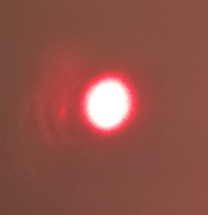
\includegraphics[width=0.235\textwidth]
      {Bilder/Auswertung/TEM00.png}}\quad
    \subfloat[$TEM_{10}$]{\label{TEM10}
      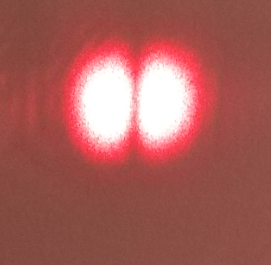
\includegraphics[width=0.25\textwidth]
      {Bilder/Auswertung/TEM10.png}}\quad
    \subfloat[$TEM_{01}$]{\label{TEM01}%
      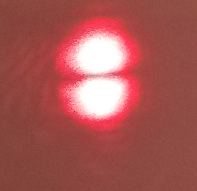
\includegraphics[width=0.25\textwidth]
      {Bilder/Auswertung/TEM01.png}}\quad
    \subfloat[$TEM_{20}$]{\label{TEM20}%
      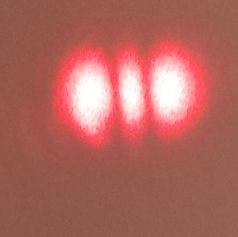
\includegraphics[width=0.25\textwidth]
      {Bilder/Auswertung/TEM20.png}}\quad
      \subfloat[$TEM_{30}$]{\label{TEM30}%
      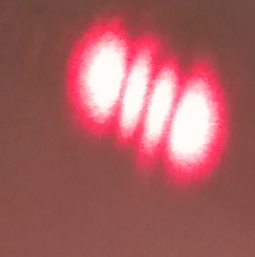
\includegraphics[width=0.25\textwidth]
      {Bilder/Auswertung/TEM30.png}}\quad
      \subfloat[$TEM_{un.}$]{\label{TEMunz}%
      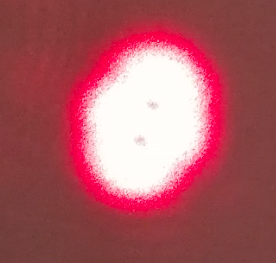
\includegraphics[width=0.25\textwidth]
      {Bilder/Auswertung/TEMunsugeordnet.png}}
      \subfloat[$TEM_{01*}$]{\label{TEM01*}\quad
      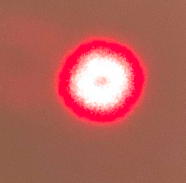
\includegraphics[width=0.245\textwidth]
      {Bilder/Auswertung/TEM11.png}}
      \caption{Transversalmoden der HeNe-Laser}
      \label{bild:Moden}
  \end{figure}

  Dabei konnten wir die klassischen $TEM$-Moden mit polarisierenden Elementen, welche die Symmetrie des Resonators aufhebt, beobachten.
  Spannenderweise kann in Abbildung \ref{TEM01*} auch eine radialsymmetrischen Mode beobachten werden. Außerdem
  gibt es eine Mode in \ref{TEMunz}, welche wir nicht identifizieren konnten. Diese könnte eine Mischmode sein.
